\section{Auswertung}

\subsection{Bestimmung der Reichweite von Alpha-Strahlung}

In dem ersten Teil des Versuchs wird die Zählrate $N$ und der Channel, damit die
Energie, in Abhängigkeit von dem Druck $p$ gemessen. Die Messzeit beträgt $t = \SI{120}{\second}$
und der Abstand bei dieser Messung beträgt $s = \SI{2.5}{\centi\meter}$. Die Messergebnisse
sind in Tabelle \ref{tab:1} dargestellt.

\begin{table}[H]
  \centering
  \caption{Messwerte bei $s =  \SI{2.5}{\centi\meter}$.}
  \label{tab:1}
  \begin{tabular}{c c c}
    \toprule
    $p \, / \, mbar$ & $N$ & Channel \\
    \midrule
    0 & 107108 &  258 \\
   50 &  80184 &  258 \\
  100 &  76867 &  258 \\
  150 &  86997 &  258 \\
  200 &  69936 &  257 \\
  250 &  65806 &  257 \\
  300 &  59917 &  257 \\
  350 &  57455 &  258 \\
  400 &  55992 &  257 \\
  450 &  53929 &  257 \\
  500 &  53846 &  257 \\
  550 &  50476 &  258 \\
  600 &  46688 &  258 \\
  650 &  44768 &  258 \\
  700 &  39064 &  257 \\
  750 &  28315 &  259 \\
  800 &   8824 &  257 \\
  850 &    180 &  257 \\
  900 &   2132 &  259 \\
  950 &    470 &  257 \\
 1013 &   2185 &  257 \\
    \bottomrule
  \end{tabular}
\end{table}

Aus den gemessenen Drücken wird nun die mittlere Reichweite der $\alpha$-Strahlung
mit der Gleichung \ref{eq:4} bestimmt. In der Abbildung \ref{abb:2} sind die Zählraten
gegen die mittlere Reichweite aufgetragen.

\begin{figure}[H]
  \centering
  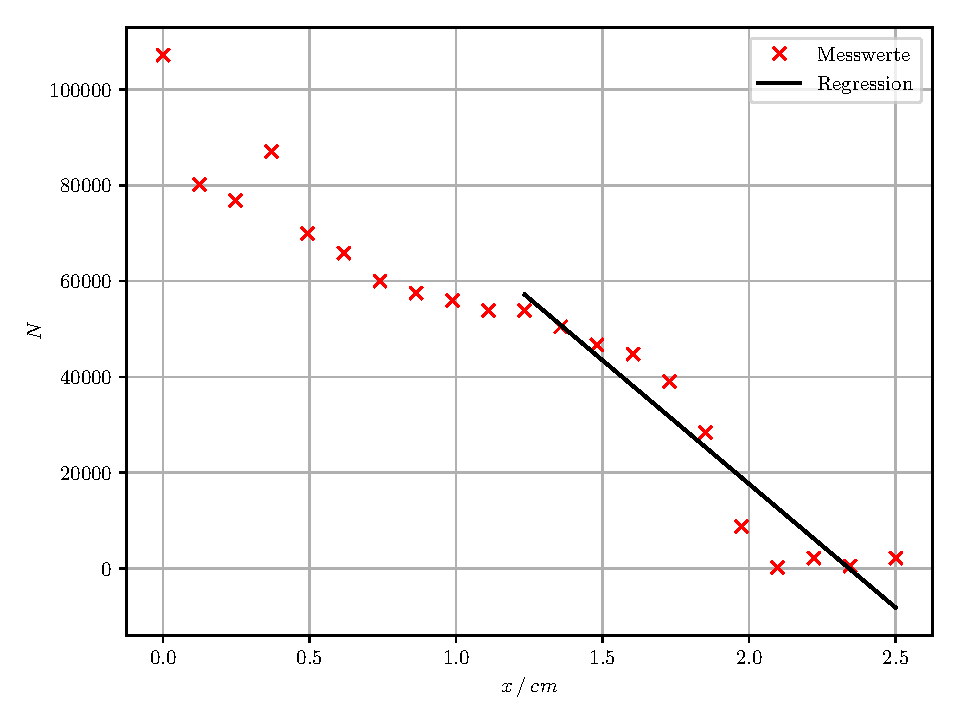
\includegraphics{plot1.pdf}
  \caption{Darstellung der Messwerte und lineare Ausgleichsrechnung.}
  \label{abb:2}
\end{figure}

Da die Zählraten ab einen bestimmten Druck linear abnehmen lässt sich eine lineare
Ausgleichsrechnung in diesem Bereich durchführen. Die Ausgleichsrechnung beginnt in
diesem Fall bei einem Druck $p = \SI{500}{\milli\bar}$ und wird mit Python 3.6
durchgeführt. Dabei ergeben sich die Parameter
der Geraden

\begin{equation}
  N = mx + b
\end{equation}

zu:

\begin{itemize}
  \item $m = \SI{-51603.60(572192)}{\per\centi\meter}$
  \item $b = \num{120842.65(1084561)}$
\end{itemize}

Nun lässt sich die mittlere Reichweite bestimmen mit der folgenden Gleichung:

\begin{equation}
  R_m = \frac{53554-b}{m}
  \label{eq:5}
\end{equation}

Dabei ist $N = 53554$ die halbe Zählrate von $p = \SI{0}{\milli\bar}$.
Der Fehler von der mittleren Reichweite lässt sich mit der Gauß´schen Fehlerfortpflanzung
bestimmen:

\begin{equation*}
  \Delta R_m = \sqrt{\left( \frac{-1}{m} \right)^2 \cdot (\Delta b)^2 +
  \left( \frac{b-53554}{m^2} \right)^2 \cdot (\Delta m )^2}
\end{equation*}

Damit ergibt sich die mittlere Reichweite zu

\begin{equation*}
  R_m = \SI{1.30(26)}{\centi\meter}.
\end{equation*}

Mit der Gleichung \ref{eq:3} lässt sich aus der mittleren Reichweite nun die Energie
bestimmen, die der mittleren Reichweite entspricht. Der Fehler dieser Energie wird
wieder mit der Gauß´schen Fehlerfortpflanzung bestimmt:

\begin{equation*}
  \Delta E_{Rm} = \sqrt{\left( \frac{1}{(3.1)}^{\frac{2}{3}}\frac{2}{3} R_m^{-\frac{1}{3}} \right)^2
  (\Delta R_m)^2}
\end{equation*}

Damit ergibt sich eine Energie von

\begin{equation*}
  E_{Rm} = \SI{0.121(16)}{\mega\eV}.
\end{equation*}

Aus dem Channel lässt sich die Energie der $\alpha$-Teilchen berechnen, da der
Channel bei $p = \SI{0}{\milli\bar}$ einer Energie $E = \SI{4}{\mega\eV}$
entspricht. Die Energie der Teilchen ist gegen die effektive Länge in
Abbildung \ref{abb:3} dargestellt.

\begin{figure}[H]
  \centering
  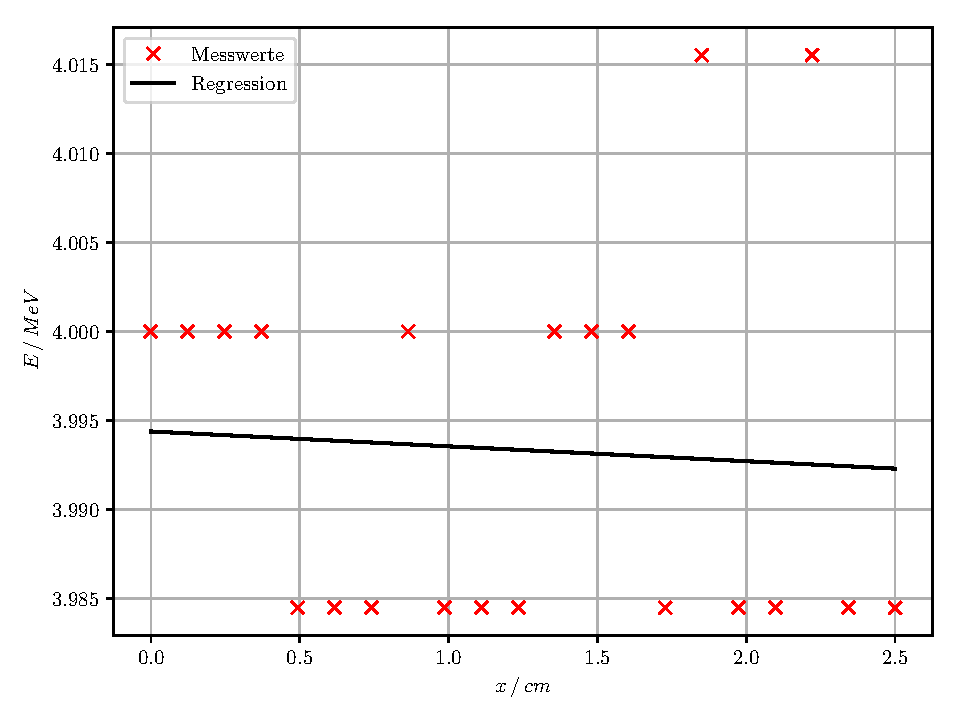
\includegraphics{plot2.pdf}
  \caption{Darstellung der Energie und lineare Ausgleichsrechnung.}
  \label{abb:3}
\end{figure}

Da die Energie linear abnehmen sollte lässt sich eine lineare Ausgleichsrechnung
durchführen. Die Ausgleichsrechnung wird wieder mit Python 3.6 durchgeführt.
Die Parameter der Geraden

\begin{equation*}
  E = mx + b
\end{equation*}

ergibt sich zu:

\begin{itemize}
  \item $m = \SI{-8.34(3124)e-4}{\mega\eV\per\centi\meter}$
  \item $b = \SI{3.994(5)}{\mega\eV}$
\end{itemize}

Der Energieverlust ergibt sich damit zu:

\begin{equation*}
  \frac{-dE}{dx} = -m = \SI{-8.34(3124)e-4}{\mega\eV\per\meter}
\end{equation*}

Als nächstes wird diese Messung wiederholt bei einem Abstand von $s = \SI{2}{\centi\meter}$.
In der Tabelle \ref{tab:2} werden die Messwerte von dieser Messung dargestellt.

\begin{table}[H]
  \centering
  \caption{Darstellung der Messwerte bei $s = \SI{2}{\centi\meter}$.}
  \label{tab:2}
  \begin{tabular}{c c c}
    \toprule
    $p \, / \, mbar$ & $N$ & Channel \\
    \midrule
    0  & 85034& 608 \\
    50 & 84100& 590 \\
    100& 82993& 582 \\
    150& 81941& 557 \\
    200& 81032& 539 \\
    250& 80118& 532 \\
    300& 78565& 512 \\
    350& 77323& 495 \\
    400& 75752& 486 \\
    450& 74062& 467 \\
    500& 71084& 455 \\
    550& 68811& 434 \\
    600& 66691& 427 \\
    650& 61738& 405 \\
    700& 57244& 398 \\
    750& 49897& 375 \\
    800& 44083& 363 \\
    850& 30164& 356 \\
    900& 23840& 355 \\
    950& 17511& 355 \\
   1013 &  9284& 355 \\
    \bottomrule
  \end{tabular}
\end{table}

Aus den verschiedenen Drücken lassen sich wieder die effektiven Längen bestimmen mit
der Gleichung \ref{eq:4}. Die Messwerte sind in Abbildung \ref{abb:4} dargestellt.

\begin{figure}[H]
  \centering
  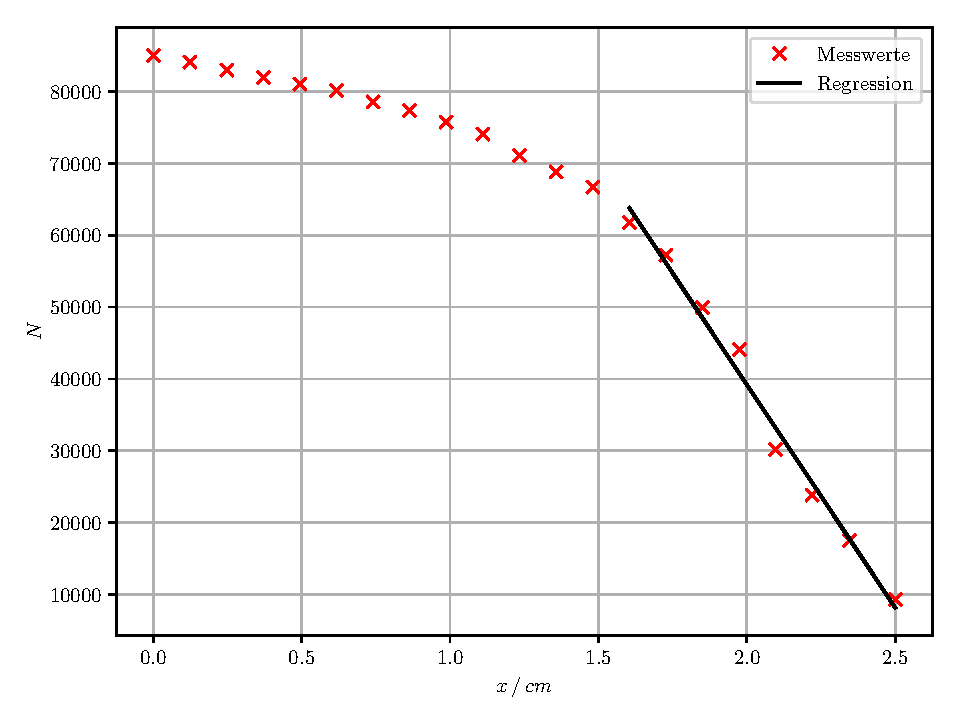
\includegraphics{plot3.pdf}
  \caption{Darstellung der Messwerte und Ausgleichsrechnung.}
  \label{abb:4}
\end{figure}

Nun lässt sich wieder eine lineare Ausgleichsrechnung ab einem Druck von $p = \SI{650}{\milli\bar}$
durchführen. Diese wird wieder mit Python 3.6 durchgeführt und die Bezeichnungen sind analog zu
den bei dem anderen Abstand. Die Parameter der Geraden ergeben sich zu:

\begin{itemize}
  \item $m = \SI{-62073.98(278811)}{\per\meter}$
  \item $b = \num{163353.65(574465)}$
\end{itemize}

Mit der Geradengleichung lässt sich wieder die mittlere Reichweite bestimmen.
Diesmal ist die halbe Zählrate $N = 42517$.
Die Rechnungen und Fehlerrechnungen sind analog zu den anderen Abstand. Damit ergibt
sich die mittlere Reichweite zu

\begin{equation*}
  R_m = \SI{1.95(13)}{\centi\meter}.
\end{equation*}

Diese mittlere Reichweite entspricht einer Energie von

\begin{equation*}
  E_{Rm} = \SI{0.158(7)}{\mega\eV}.
\end{equation*}

Aus den ermittelten Channel lässt sich wieder die Energie bestimmen. Die Energie
als Funktion der effektiven Länge ist in Abbildung \ref{abb:5} dargestellt.

\begin{figure}[H]
  \centering
  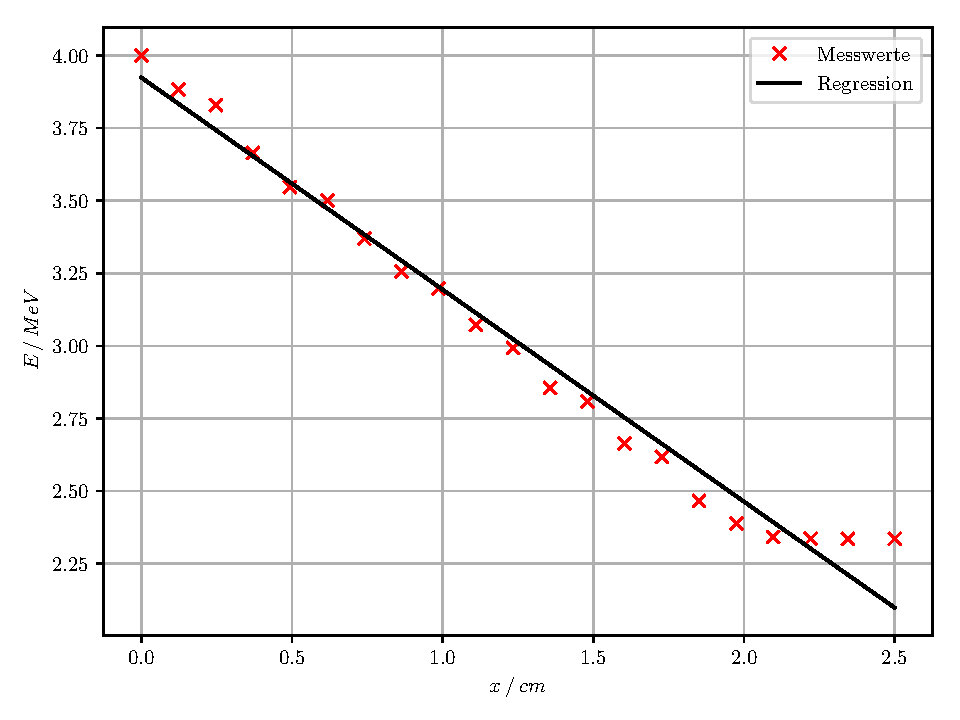
\includegraphics{plot4.pdf}
  \caption{Darstellung der Energie und lineare Ausgleichsrechnung.}
  \label{abb:5}
\end{figure}

Nun wird wieder eine lineare Ausgleichsrechnung durchgeführt um eine Funktion
für die Energie zu erhalten. Die Parameter der Geraden ergeben sich zu:

\begin{itemize}
  \item $m = \SI{-0.730(24)}{\mega\eV\per\centi\meter}$
  \item $b = \SI{3.924(35)}{\mega\eV}$
\end{itemize}

Damit ergibt sich ein Energieverlust von

\begin{equation*}
  -\frac{dE}{dx} = \SI{0.730(24)}{\mega\eV\per\centi\meter}.
\end{equation*}

\subsection{Statistik des radioaktiven Zerfalls}

Nun werden die Zählraten bei einem Druck von $p = \SI{0}{\milli\bar}$ 100 mal gemessen
bei einer Messzeit von $t = \SI{10}{\second}$. Die Messergebnisse sind in Tabelle \ref{tab:3}
dargestellt.

\begin{table}[H]
  \centering
  \caption{Messwerte der Zählraten für die Statistik des radioaktiven Zerfalls.}
  \label{tab:3}
  \begin{tabular}{c c c c c}
    \toprule
    N & N & N & N & N \\
    \midrule
    6993 & 6959 & 6529 & 6741 & 6875 \\
    6622 & 6900 & 7055 & 6772 & 6842 \\
    6776 & 6896 & 6378 & 6247 & 6789 \\
    6484 & 6562 & 6847 & 6952 & 6822 \\
    6369 & 6710 & 6582 & 6956 & 6539 \\
    6757 & 6490 & 6353 & 6912 & 6459 \\
    6911 & 6451 & 6933 & 6777 & 6566 \\
    6303 & 6955 & 6811 & 6288 & 6999 \\
    6449 & 6531 & 6935 & 6889 & 6868 \\
    6634 & 6315 & 6355 & 6357 & 6835 \\
    6463 & 6774 & 6711 & 6643 & 6624 \\
    6612 & 6466 & 6837 & 6362 & 6612 \\
    6873 & 6468 & 6652 & 6952 & 6705 \\
    6438 & 6366 & 6804 & 6641 & 6499 \\
    6711 & 6417 & 6204 & 6666 & 6903 \\
    6508 & 6743 & 6567 & 6653 & 6481 \\
    6402 & 6470 & 6900 & 6324 & 6776 \\
    6682 & 6768 & 6202 & 6568 & 6990 \\
    6705 & 6671 & 6796 & 6633 & 6689 \\
    6349 & 6821 & 7033 & 6703 & 6788 \\
    \bottomrule
  \end{tabular}
\end{table}

Diese Messwerte werden nun in einem Histogramm aufgetragen und mit einer Gauß- und
Poissonverteilung verglichen. Das ist in Abbildung \ref{abb:6} gezeigt.
Damit die Varianz nicht zu groß ist wird jeder Wert durch 100 geteilt.

\begin{figure}[H]
  \centering
  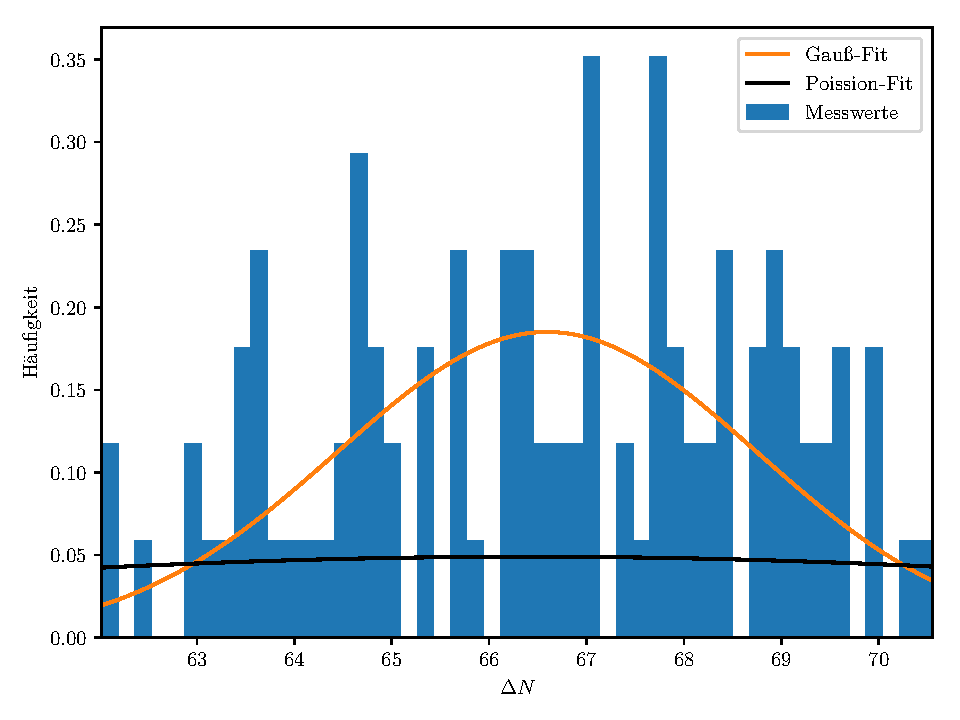
\includegraphics{plot5.pdf}
  \caption{Histogramm der Messwerte mit einer Gauß- und einer Poissonverteilung.}
  \label{abb:6}
\end{figure}

Außerdem lassen sich aus den Messwerten der Mittelwert und deren Varianz von einer
Gaußverteilung mit den folgenden Gleichungen bestimmen.

\begin{equation*}
    \bar{x} = \frac{1}{N} \sum_{i=1}^{N} x_i
\end{equation*}

\begin{equation*}
  V_g = \frac{1}{N(N-1)} \sum_{i}(x_i-\bar{x})^2
\end{equation*}

Damit ergibt sich für den Mittelwert und die Varianz für eine Gaußverteilung:

\begin{itemize}
  \item $\bar{N} = \num{66.60}$
  \item $V_p = \num{4.646}$
\end{itemize}

Von einer Poissonverteilung der Form

\begin{equation*}
  P(N, \lambda) = \frac{\lambda^N}{N!} \exp{(-\lambda)}
\end{equation*}

ist die Varianz

\begin{equation*}
  V_p = \lambda.
\end{equation*}

Damit ergibt sich die Varianz der Poissonverteilung zu

\begin{equation*}
  V_p = 66,87.
\end{equation*}
